\documentclass[12pt]{article}

% Language setting
% Replace `english' with e.g. `spanish' to change the document language
\usepackage[english]{babel}

% Set page size and margins
% Replace `letterpaper' with `a4paper' for UK/EU standard size
\usepackage[letterpaper,top=2cm,bottom=2cm,left=3cm,right=3cm,marginparwidth=1.75cm]{geometry}

% Useful packages
\usepackage{amsmath}
\usepackage{graphicx}
\usepackage[colorlinks=true, allcolors=blue]{hyperref}

\usepackage{listings}
\usepackage{xcolor}

\definecolor{codegray}{rgb}{0.9,0.9,0.9}
\definecolor{keywordcolor}{rgb}{0.0,0.0,1.0}
\definecolor{commentcolor}{rgb}{0.5,1.0,0.5}
\definecolor{stringcolor}{rgb}{1.0,0.0,0.82}

\lstdefinestyle{mystyle}{
    backgroundcolor=\color{codegray},   
    commentstyle=\color{commentcolor},
    keywordstyle=\color{keywordcolor}\bfseries,
    stringstyle=\color{stringcolor},
    basicstyle=\ttfamily\footnotesize,
    breakatwhitespace=false,         
    breaklines=true,                 
    captionpos=b,                    
    keepspaces=true,                 
    numbers=left,                    
    numbersep=5pt,                  
    showspaces=false,                
    showstringspaces=false,
    showtabs=false,                  
    tabsize=4
}

\lstset{style=mystyle}

\begin{document}

\title{CS726 Programming Assignment 3 \\ LLM Sampling and Decoding Techniques}
\author{Kshitij Vaidya \\ Raunak Mukherjee \\ Anshu Arora}
\date{\today}
\maketitle

\tableofcontents
\clearpage

\section{Task 0 : Introduction to LLM Decoding}

To familiarise ourselves with the decoding techniques in Large Language Models, we implemented functions to translate Hindi to English using the Llama-2 model and the data was used from the IN22-Gen dataset. The \textbf{BLEU} and \textbf{ROUGE} scores were used for evaluation of the translations.

\subsection{Decoding Techniques} 

\begin{enumerate}
    \item \textbf{Greedy Decoding} : Here, at every step we select the token with the highest probability from the output distribution of the LLM. Mathematically, we represent this as :
    \begin{equation}
        \hat{y}_t = \arg\max_{y_t} P(y_t | y_{<t}, x)
    \end{equation}
    where $\hat{y}_t$ is the token selected at time step $t$ and $y_{<t}$ is the sequence of tokens selected till time step $t-1$. This sequence repeats till we reach an EOS token or the maximum output length of the sequence.

    \item \textbf{Random Sampling with Temperature} : Here, we randomly sample from the probability distribution of the output tokens. The sharpness of the distribution is controlled by the temperature parameter $\tau$. We first modify the distribution as :
    \begin{equation}
        P'(w|y_{<t}, x) = \displaystyle\frac{P(w|y_{<t}, x)^{1/\tau}}{\sum_{w'} P(w'|y_{<t}, x)^{1/\tau}}
    \end{equation}
    and then sample from this distribution. Here, higher values of $\tau$ lead to a more uniform distribution and lower values lead to a sharper distribution. Thus, lower values of $\tau$ lead to more deterministic sampling and perform similar to Greedy Decoding.

    \item \textbf{Top-K Sampling} : We restrict our choices to the K most probable tokens in the distribution. We first sort the tokens in decreasing order of probability and then sample from the top-K tokens. This is mathematically represented as :
    \begin{equation}
        V_k = \{ w_1, w_2 \cdots w_k \}, where P(w_i) \geq P(w_{i+1}) for i < k
    \end{equation}
    The probabilities are then normalised and we select the token by sampling from this distribution

    \item \textbf{Nucleus Sampling} : We take the smallest set of tokens whose cumulative probability is greater than a threshold $p$. We first sort the tokens in decreasing order of probability and then select the smallest set of tokens whose cumulative probability is greater than $p$. This is mathematically represented as :
    \begin{equation}
        V_p = \{ w | \sum_{w' \in V_p} P(w') \geq p \}
    \end{equation}
    The probabilities are then normalised and we select the token by sampling from this distribution
\end{enumerate}

\subsection{Evaluation Metrics}

\begin{enumerate}
    \item \textbf{BLEU Score} : The BLEU score is a metric used to evaluate the quality of machine-translated text. It is based on the n-gram precision of the translated text. The BLEU score is calculated as :
    \begin{equation}
        \text{BLEU} = \text{BP} \times \exp\left(\sum_{n=1}^{N} w_n \log p_n\right)
    \end{equation}
    where $p_n$ is the n-gram precision and $w_n$ is the weight assigned to the n-gram precision. The brevity penalty $BP$ is used to penalise shorter translations.

    \item \textbf{ROUGE Score} : The ROUGE score is a metric used to evaluate the quality of summaries. It is based on the overlap of n-grams between the generated summary and the reference summary. The ROUGE score is calculated as :
    \begin{equation}
        \text{ROUGE} = \frac{\sum_{n=1}^{N} \text{ROUGE}_n}{N}
    \end{equation}
    where $\text{ROUGE}_n$ is the n-gram overlap between the generated summary and the reference summary.
\end{enumerate}


\subsection{Results}

\begin{table}[htbp]
    \centering
    \begin{tabular}{|lcccc|}
        \hline
        \textbf{Method} & BLEU & ROUGE-1 & ROUGE-2 & ROUGE-LCS \\
        \hline
        Greedy & 0.3099 & 0.3543 & 0.1296 & 0.2710 \\
        \hline
        Random ($\tau = 0.5$) & 0.2928 & 0.2932 & 0.0931 & 0.2266 \\
        Random ($\tau = 0.9$) & 0.1985 & 0.2000 & 0.0585 & 0.1647 \\
        \hline
        Top-k ($k = 5$) & 0.2476 & 0.2464 & 0.0698 & 0.1826 \\
        Top-k ($k = 10$) & 0.2490 & 0.2584 & 0.0797 & 0.1984 \\
        \hline
        Nucleus ($p = 0.9$) & 0.0846 & 0.1473 & 0.0422 & 0.1153 \\
        \hline
    \end{tabular}
    \caption{Comparison of different decoding methods using BLEU and ROUGE scores}
    \label{tab:decoding_comparison}
\end{table}

\begin{figure}[htbp]
    \centering
    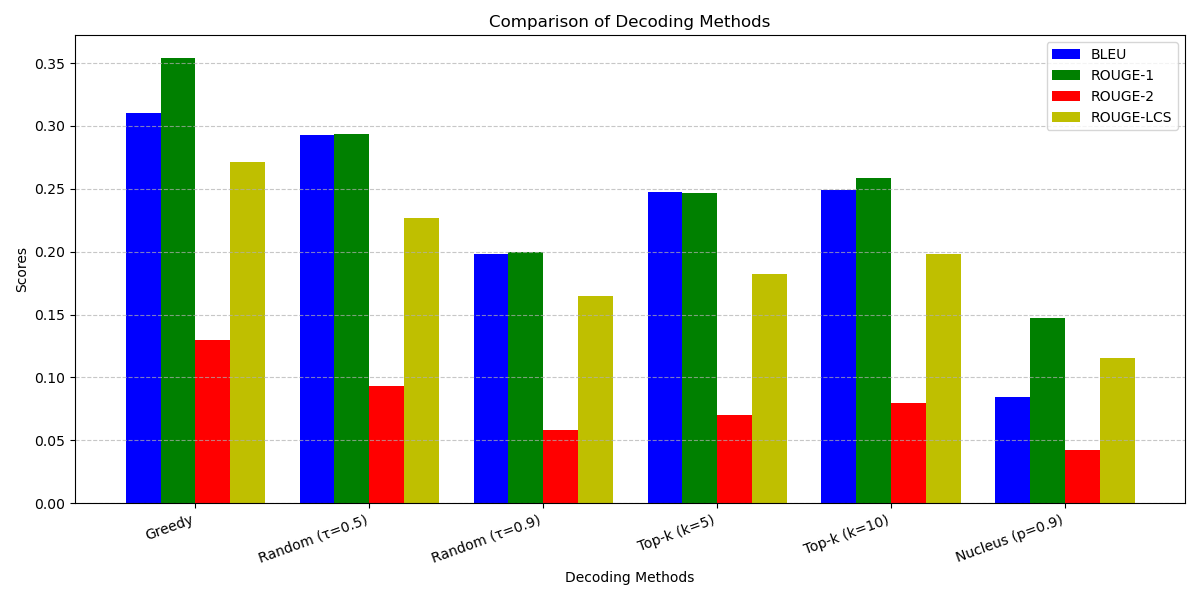
\includegraphics[width=0.8\textwidth]{decoding_methods.png}
    \caption{Comparison of different decoding methods using BLEU and ROUGE scores}
    \label{fig:decoding_comparison}
\end{figure}

\newpage

\section{Task 1 : Word-Constrained Decoding}

\noindent Here, a variant of Grammar-Constrained Decoding is used which is called Word Constrained Decoding. In this, we are given a set of words that must appear in the output sequence. We implement a greedy decoding technique that takes this set of words in account improves the LLM performance. We use a Trie based implementation to store the set of words and use it to check if the word is present in the output sequence. The algorithm is as follows :

\begin{enumerate}
    \item We build the Trie using the set of words that must appear in the output sequence.
    \item We then initialise the output sequence as an empty list and the current word as an empty string.
    \item We then iterate over the output sequence and check if the current word is present in the Trie. If it is present, we add the current word to the output sequence and reset the current word to an empty string.
    \item If the current word is not present in the Trie, we add the current token to the current word and continue.
    \item We repeat this process till we reach the end of the output sequence.
\end{enumerate}

\subsection{Trie Implementation}

The following Python code implements a Trie data structure to manage a word list. The Trie efficiently supports insertion, prefix checking, and word completion validation.

\begin{lstlisting}[language=Python, caption=Trie Implementation]
from collections import defaultdict

class TrieNode:
    def __init__(self):
        self.children = defaultdict(TrieNode)
        self.isEndOfWord = False
    
class Trie:
    def __init__(self, tokenizer):
        self.root = TrieNode()
        self.tokenizer = tokenizer
    
    def insert(self, word):
        tokens = self.tokenizer.encode(word, add_special_tokens=False)
        node = self.root
        for token in tokens:
            node = node.children[token]
        node.isEndOfWord = True
    
    def startsWith(self, prefixTokens):
        node = self.root
        for token in prefixTokens:
            if token not in node.children:
                return False
            node = node.children[token]
        return True

    def validCompletion(self, prefixTokens) -> bool:
        node = self.root
        for token in prefixTokens:
            if token not in node.children:
                return False
            node = node.children[token]
        return node.isEndOfWord
\end{lstlisting}

\subsection{Results}

\noindent The word constrained decoding technique and the greedy decoding technique were used to translate Hindi to English. The BLEU and ROUGE scores were used for evaluation of the translations. The results show that this method performs better then the greedy decoding technique marginally. The BLEU and ROUGE scores are as follows :

\begin{table}[htbp]
    \centering
    \begin{tabular}{|l|c|}
        \hline
        \textbf{Metric} & \textbf{Score} \\
        \hline
        BLEU & 0.19298 \\
        ROUGE-1 & 0.43248 \\
        ROUGE-2 & 0.27158 \\
        ROUGE-LCS & 0.39884 \\
        \hline
    \end{tabular}
    \caption{Task 1 - BLEU and ROUGE Scores}
    \label{tab:task1_scores}
\end{table}

\begin{figure}[htbp]
    \centering
    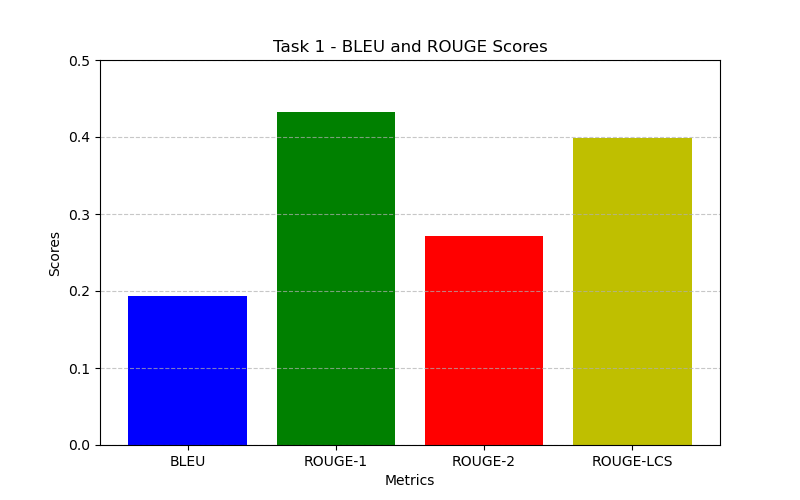
\includegraphics[width=0.8\textwidth]{task1.png}
    \caption{Task 1 - BLEU and ROUGE Scores}
    \label{fig:task1_scores}
\end{figure}

\newpage

\section{Task 2 : Staring into Medusa's Heads}

\bibliographystyle{plain}
\bibliography{references}

\end{document}